\secnumbersection{MARCO CONCEPTUAL}

Se debe describir la base conceptual o fundamentos en los que se basa tu memoria, es decir, todos los conceptos técnicos, metodologías, herramientas, etc. que están involucradas en la solución propuesta. En el fondo esta parte permite precisar y delimitar el problema, estableciendo definiciones para unificar conceptos y lenguaje y fijar relaciones con otros trabajos o soluciones encontradas por otros al mismo problema evitando así plagios o repetir errores ya conocidos o abordados por otros.

En esta parte es importante relacionar estos conceptos con la memoria y es fundamental utilizar referencias bibliográficas (o de la web) recientes, por ejemplo \cite{gettelfinger2004will}.
\subsection{CONCEPTOS TÉCNICOS}

\subsubsection{\textit{SOFTWARE AS A SERVICE (SaaS)}} 

El software como servicio o SaaS (Software as a Service, en inglés) es un tipo de servicio de cloud computing que se enfoca en la entrega de software basado en la nube, para esto se necesita un proveedor de servicios de nube que desarrolla y mantiene el software de las aplicaciones, proporciona actualizaciones automáticas y lo pone a disposición de sus clientes a través de Internet con un sistema de pago por uso. De este modo, los clientes del SaaS reducen sus costos.\footnote{\href{https://www.oracle.com/applications/what-is-saas/}{Oracle - What is SaaS?}}

\subsubsection{\textit{WEB FRAMEWORKS}}

En los inicios del desarrollo web todas las aplicaciones eran programadas “a mano”, lo que provocaba muchos errores. Para poder superar estas dificultades se introdujeron los Web Frameworks en los inicios de la década de los 2000. Los webs frameworks son herramientas que ayudan a construir un sitio web disminuyendo bugs, errores y tiempo. Los frameworks se dividen principalmente en dos categorías: Front-end y Back-end. \cite{analysiswf} 

\subsubsubsection{\textit{FRONT-END}}

También conocido como \textit{client-side}, es el componente de la aplicación o página web con el que el usuario interactúa. Incluye lo que el usuario ve como imágenes, botones, colores, gráficos, tablas, entre otros. HTML y CSS son usados para el diseño y estilo, mientras que JavaScript se utiliza para validaciones, animaciones, cambios de estado, etc. El rendimiento y la sensibilidad son los 2 grandes objetivos del desarrollo front-end. El desarrollador se asegura que la aplicación sea sensible, es decir, que se muestren las vistas correctamente en diferentes pantallas como las de monitor, celular, tablets. \cite{webframedbws}

\subsubsubsection{\textit{BACK-END}}

En \textit{back-end} las preocupaciones son otras, por ejemplo, protección de APIs de ataques externos, autenticar usuarios, interacción con bases de datos y manejar solicitudes de usuarios. Los back-end frameworks son evaluados según sus métodos de programación, lenguajes que soporta e interfaces. También, proveen herramientas y plantillas que ayudan a los desarrolladores en varias tareas del desarrollo. \cite{webframedbws}

\subsubsection{\textit{APPLICATION PROGRAMING INTERFACE (API)}}

\textit{Application Programming Interface} (API) es un conjunto de herramientas, definiciones y protocolos que se utiliza para que los productos y servicios se comuniquen con otros, sin tener que diseñar permanentemente una infraestructura de conectividad nueva. Las API pueden ser privadas (para uso interno), compartidas (con terceros para brindar flujos de ingresos adicionales) o públicas (entidades externas pueden desarrollar aplicaciones que interactúen con sus API para fomentar la innovación).
El propósito de las API es la integración, es decir, se encargan de conectar los datos, las aplicaciones y los dispositivos para que todas las tecnologías puedan comunicarse y trabajar mejor en conjunto.

\subsubsubsection{API REST}

REST es una sigla que significa \textit{REpresentational State Transfer}, es un término acuñado por Roy Fielding presentado en su tesis doctoral \cite{fieldingapi}, y lo define como un estilo de arquitectura para sistemas distribuidos de hipermedia, describiendo las restricciones de ingeniería de software que guían REST. Estas restricciones son las siguientes:
\begin{itemize}
    \item \textbf{Arquitectura cliente-servidor:} La separación de responsabilidades es el principio detrás de esta restricción. Cuanto menos conoce el servidor del cliente, y viceversa, resulta más fácil el cambio de componentes.
    \item \textbf{Ausencia de estado:} La comunicación debe ser sin estado por naturaleza, es decir, cada petición del cliente al servidor debe contener solo la información necesaria para entender la petición y no puede tomar ventaja de ningún contexto almacenado en el servidor. Por esto, las sesiones se deben mantener en el cliente.
    \item \textbf{Caché:} La data de una response a una petición debe estar implícita o explícitamente etiquetada como cacheable o no cacheable. Si las respuestas es cacheable, se pueden enviar respuestas cacheadas desde cualquier punto de la red sin necesidad que la petición llegue al servidor.
    \item \textbf{Sistema por capas:} Tiene relación con la separación de responsabilidades y establece que un cliente debe conocer únicamente la capa a la que le está hablando.  Es decir, no debe saber qué bases de datos se está utilizando, cachés, proxies, etc.
    \item \textbf{Interfaz uniforme:} La principal característica que distingue la arquitectura REST de otras es el énfasis de una interfaz uniforme entre componentes, para que la información se transfiera de forma estandarizada. 
    \item \textbf{Código bajo demanda:} REST permite extender la funcionabilidad del cliente mediante la descarga y ejecución de código en forma de scripts. 
\end{itemize}
REST es un estilo de arquitectura no un estándar, es por esto, que las API REST suelen llamarse API RESTful, es decir, una API que sigue la arquitectura REST. Puede resultar complejo implementar todos los principios de REST en una API, por ello, el modelo de madurez de Richardson (Fowler, 2010) que describe cuanto se apega un servicio a las características de REST. Posee cuatro niveles:
\begin{itemize}
    \item \textbf{Nivel 0:} El servicio cuenta con una sola URI que acepta todo el rango de operaciones, con unos recursos poco definidos.
    \item \textbf{Nivel 1:} El servicio cuenta con varias URIs para distintos recursos. Necesita saber qué tipo de operación realizar a través de la URI o el payload.
    \item \textbf{Nivel 2:} El servicio hace uso de las URIs para recursos identificando la operación a través de los métodos HTTP. Además, hace un correcto uso de los códigos de estado.
    \item \textbf{Nivel 3:} El servicio implementa Hypermedia as the engine of application state (HATEOAS).
\end{itemize}
Los servicios que alcancen el nivel 3 podrán ser considerados como API RESTful.

\subsection{HERRAMIENTAS TECNOLÓGICAS}

\subsubsection*{\textit{AMAZON WEB SERVICES (AWS)} }

Amazon Web Services\footnote{\href{https://aws.amazon.com/es/what-is-aws/}{¿Qué es AWS?}}, o AWS, es la plataforma en la nube más utilizada en el mundo, que cuenta con una cantidad de servicios y características ofreciendo desde tecnologías de infraestructura como cómputo, almacenamiento y bases de datos hasta tecnologías emergentes como aprendizaje automático e inteligencia artificial, data lakes e Internet of Things. Dentro de los servicios más importantes están:
\begin{itemize}
    \item \textbf{EC2:} \textit{Amazon Elastic Compute Cloud} ofrece capacidad de computación con más de 500 instancias y la posibilidad de elegir procesador, almacenamiento, redes, sistema operativo y modelo de compra para ajustar a las necesidades del usuario.
    \item \textbf{S3:} \textit{Amazon Simple Storage Service} es un servicio de almacenamiento de objetos que ofrece escalabilidad, disponibilidad de datos y un gran rendimiento. Por las clases de almacenamiento y características de administración fáciles de usar, es posible optimizar costos, organizar datos y configurar controles de acceso.
    \item \textbf{RDS:} \textit{Amazon Relational Database Service} es una colección de servicios administrados que facilita las tareas de configuración, operación y escalado de una base de datos en la nube. Se puede elegir entre motores como Amazon Aurora, MySQL, PostgreSQL, MariaDB, SQL Server, entre otros.
    \item \textbf{Lambda:} Servicio informático sin servidor (serverless) y basado en eventos que permite ejecutar código para cualquier tipo de aplicación o servicio back-end sin la necesidad de servidores.
\end{itemize}

\subsubsection{\textit{JAVASCRIPT}}

JavaScript, o JS, es un lenguaje de programación orientado a objetos, utilizado mayormente para el desarrollo web en ambos \textit{front-end} y \textit{back-end}. JS tiene una gran comunidad, contiene un conjunto de bibliotecas de código abierto que facilitan tareas para el desarrollador como la visualización de datos y comunicación con el usuario.

\subsubsubsection{\textit{NODE.JS}}

Node.js es un entorno en tiempo de ejecución asíncrono basado en eventos diseñada para desarrollar, mayormente, en server-side. Soporta el manejo de muchas conexiones al mismo tiempo. Node.js tiene propiedades que lo hacen escalable. Usa el motor V8 de Google para ejecutar código de JavaScript transformándolo en código máquina y optimiza mediante métodos complicados. \cite{webframedbws}

\subsubsubsection{\textit{REACTJS}}

ReactJS es una biblioteca de JavaScript para el desarrollo de interfaces de usuarios dinámicas. Creado y mantenido por Facebook. Interfaces complejas pueden ser compuestas de piezas pequeñas, isoladas y reusables de código llamadas “componentes”. ReactJS usa JSX, preprocesador que agrega sintaxis XML a JavaScript, para la escritura simple de HTML. \cite{webframedbws}

\subsubsection{\textit{JAVA}}

Java\footnote{\href{https://www.ibm.com/cloud/learn/java-explained}{What is Java? | IBM}} es un lenguaje de programación orientado a objetos lanzado en el año 1995 por Sun Microsystems. Una de las mayores ventajas del desarrollo con Java es su portabilidad, independiente en que dispositivo se programe Java se podrá correr en otros dispositivos.
Java es una tecnología que consiste en el lenguaje de programación y una plataforma de software. Para crear aplicaciones con Java se necesita descargar el Java Development kit (JDK). Se escribe el código, luego un compilador lo transforma a Java bytecode que corre en la Java Virtual Machine (JVM). Cualquier sistema que soporte JVMs puede correr aplicaciones Java.

\subsubsubsection{\textit{JAVASERVER FACES}}

JavaServer Faces\footnote{\href{https://www.juntadeandalucia.es/servicios/madeja/contenido/recurso/101}{JavaServer Faces (JSF)}} (JSF) es una infraestructura de interfaz de usuario o de APIs que facilita el desarrollo de aplicaciones web de Java. JSF usa principalmente JavaServer Pages (JSP) para el despliegue de las páginas. Los principales componentes son:
\begin{itemize}
    \item Una API para representar componentes de interfaz de usuario y gestionar su estado.
    \item Dos bibliotecas de etiquetas JSP para expresar componentes en una página JSP y enlazar los componentes a objetos del servidor.
\end{itemize}
Una de las grandes ventajas de JSF es la clara separación entre el comportamiento y la presentación, esto permite que cada desarrollador de un equipo se enfoque en su parte del proceso de desarrollo, y proporciona un modelo de programación sencillo para enlazar las piezas. No obstante, en comparación con otros entornos o arquitecturas, no es muy rápida.

\subsection{ESTADO DEL ARTE}
La tecnología de WiseConn permite a los administradores de campo poder monitorear, controlar y automatizar de manera inalámbrica los sistemas de riego para aumentar los ingresos, disminuir los gastos y ayudar a administrar el tiempo.

En terreno, una red de nodos inteligentes se conectan a sensores y actuadores recopilando información de clima, humedad de suelo, riego, nutrición, entre otros. Estos nodos se comunican entre si por medio de señales de radio enviando la información a la nube, donde es almacenada y gestionada por servidores en \textit{Amazon Web Services}. Los datos se despliegan en Dropcontrol para su análisis en tiempo real, simplificando las tareas de riego reduciendo costos de mano de obra, agua y energía.
\begin{figure}[h]
	\centering
	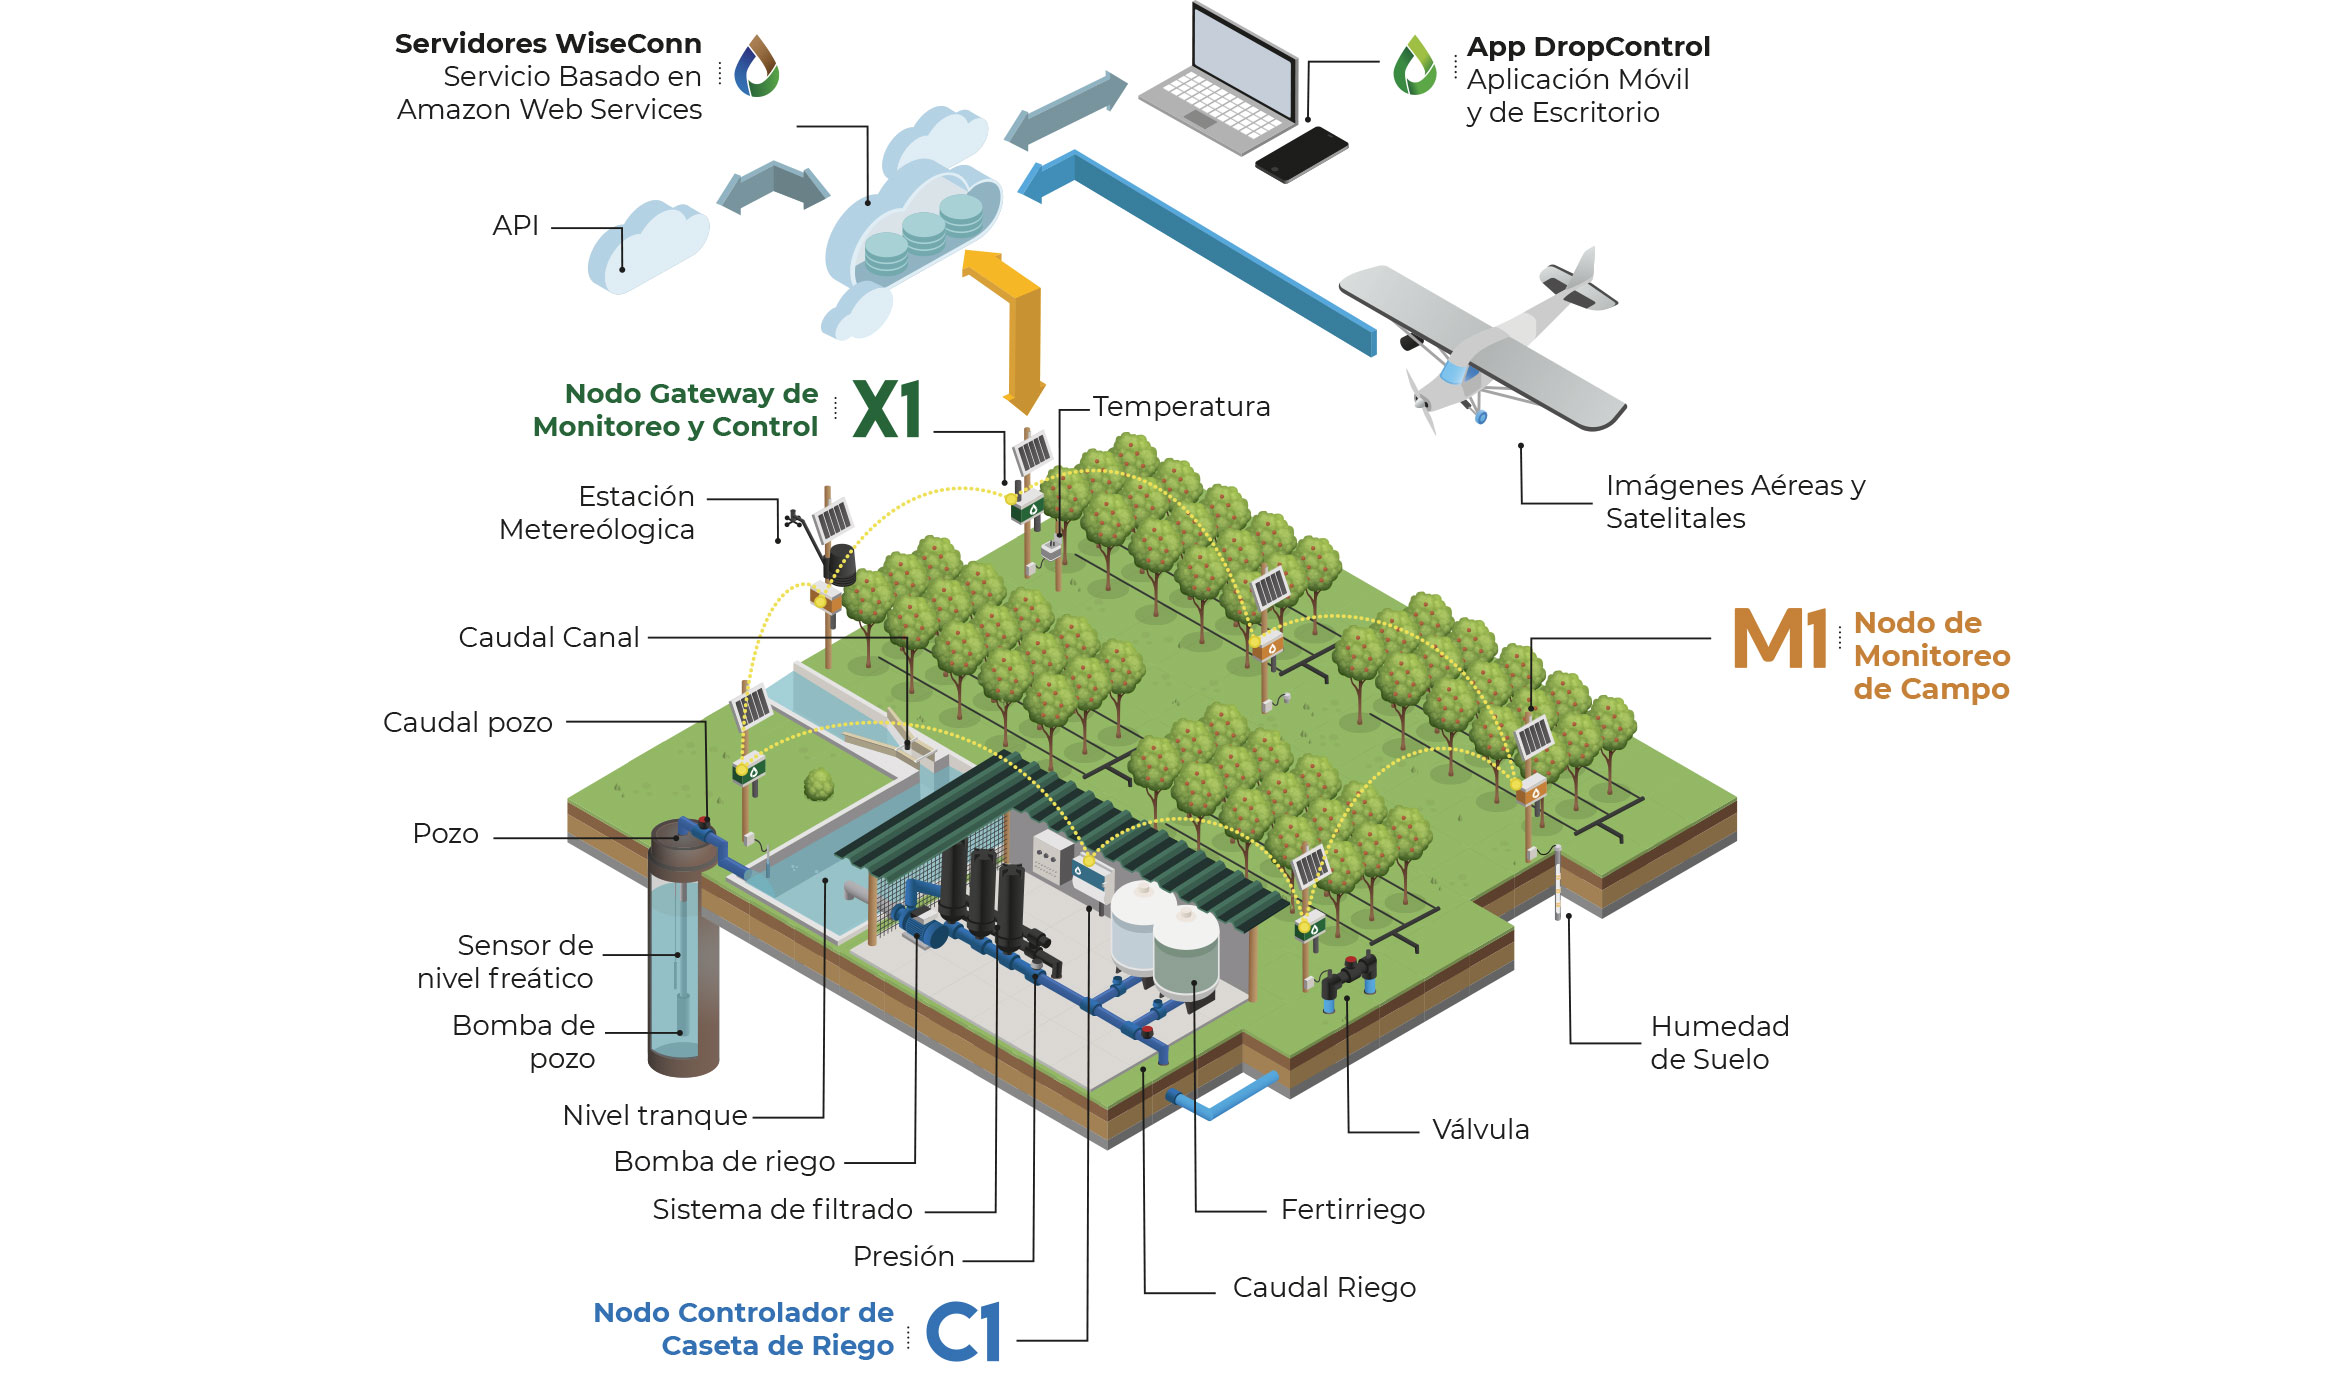
\includegraphics[width=0.8\textwidth]{mundo_dropcontrol}
	\caption{\label{fig:mundrop} ¿Cómo funciona DropControl?}
\end{figure}

\subsubsection{COMPETENCIAS EN EL MERCADO}

\subsubsection{NETAFIM}

